\begin{frame}{\tHq ditau hadhad channel selection}
  \begin{columns}
    \begin{column}{0.5\textwidth}
      \centering 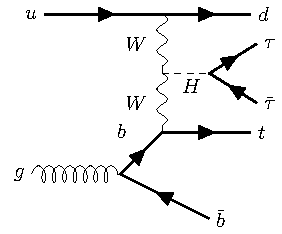
\includegraphics[width=0.7\textwidth]{tHq_tautau}\\
      %\includegraphics[width=0.45\textwidth]{/cephfs/user/s6chkirf/feynman_diagrams/tHq_WW}
      %\includegraphics[width=0.45\textwidth]{/cephfs/user/s6chkirf/feynman_diagrams/tHq_ZZ}
      \begin{itemize}
        \item n-jets: 2 (b-jets: \textbf{1})
        \item b-jet WP: 70 DL1r
        \item nLeptons \& nTaus: \bf{$1e / \mu~2\tau_{\text{had}}$}
        \item $E_{\text{T,miss}}$: no cut (to \SI{800}{GeV})
      \end{itemize}
    \end{column}
    \begin{column}{0.7\textwidth}
      \vspace*{-0.05\textwidth}
      \begin{itemize}
        \footnotesize
        \item jets:
        \vspace*{-0.02\textwidth}
        \begin{itemize}
          \footnotesize
          \item $p_T>\SI{35}{GeV}$
          \item $|\eta|<4.5$
          \item EMPFlow
        \end{itemize}
        \item electrons:
        \vspace*{-0.02\textwidth}
        \begin{itemize}
          \footnotesize
          \item $p_T>\SI{20}{GeV}$ leading \SI{27}{GeV}
          \item $|\eta|<2.5$ not in 1.37 - 1.52
          \item WP: LooseAndBLayerLH ; \\isolation: no requirement
        \end{itemize}
        \item muons:
        \vspace*{-0.02\textwidth}
        \begin{itemize}
          \footnotesize
          \item $p_T>\SI{20}{GeV}$ leading \SI{27}{GeV}
          \item $0.01<|\eta|<2.5$
          \item WP: Loose ; isolation: no requirement
        \end{itemize}
        \item taus:
        \vspace*{-0.02\textwidth}
        \begin{itemize}
          \footnotesize
          \item $p_T>\SI{20}{GeV}$ leading \SI{27}{GeV}
          \item $|\eta|<2.5$ not in 1.37 - 1.52
          \item WP: RNNLoose
          \item ASG recommended OLR ($\tau_{had}$ remove jets)
        \end{itemize}
      \end{itemize}
    \end{column}
  \end{columns}
\end{frame}
  
